%% LaTeX2e class for student theses
%% sections/content.tex
%% 
%% Karlsruhe Institute of Technology
%% Institute for Program Structures and Data Organization
%% Chair for Software Design and Quality (SDQ)
%%
%% Dr.-Ing. Erik Burger
%% burger@kit.edu
%%
%% Version 1.3.5, 2020-06-26

\chapter{Feature generation}
\label{ch:features}
%% ==============
Artificial neural networks(ANNs) and other machine learning techniques have strict requirements to their input data.
For ANNs specifically, the input needs to be of fixed size and ideally as low dimensional as possible.
To achieve that, a fixed number of features are extracted from the molecules.
In order to learn, all the data required to predict molecular properties, in this case the activation barrier, should be encoded in the features.
These features can then be used to train a neural network.

Simple encoders extract well know features of molecules such as their mean electro negativity or atomic numbers \cite{LO20181538}.
Approaches by state-of-the-art chemical encoders include using graph convolutions to parse the chemical structure into fixed size features \cite{GNN_ENCODER}.
Others try to encode interaction of different atoms or species of atoms into their features \cite{PhysRevLett.108.058301}.
The feature generators relevant to this project are spacial encoders.

Spacial encoders in chemistry generally focus on describing the interaction of chemical elements within a certain radius, rather 
than the space itself \cite{Bart_k_2013}.
Since global rotation and translation of an element generally does not influence its chemical properties,
encoders try to produce rotationally invariant representations.
This usually limits the possibilities of reconstructing the input data.
A 3D representation can therefore not easily be computed from the generated features.

The feature generators proposed here have the ability to partly reconstruct the 3D space they are encoding.
In order to retain partial rotational invariance the special structure of the input data is used.
All catalyst molecules in the dataset have a central metal atom and a reaction pocket composed of a hydrogen atom attached to the metal center.
By the centers of these 2 atoms a unique axis is formed.
This axis is used to align the molecules.

The use of this special structure of catalyst molecules to generate partly invariant features seems to be a novel approach.

After alignment, two different approaches to feature generation are explored.
The first method slices the molecule at certain heights.
The slices are then described using a fully rotationally invariant descriptor.

The second approach uses a combination of different 3D basis functions to encode the space surrounding the central atom.
Since this description is not fully invariant, data augmentation is used along the remaining axes of freedom.

\section{Alignment of catalyst molecules}

Every catalyst molecule $\mathbb{E}$ in the dataset has a central Iridium atom with position $p_{Ir} \in \mathbb{E}$.
The Iridium atom is set to the center, all other atoms are aligned accordingly.

$$ \forall p_i \in \mathbb{E}: p_i' = p_i - p_{Ir}$$

Now that the element is centered, the next step is to rotate it.
Every catalysts has a reaction pocket attached to the central metal atom.
This reaction pocket is defined by a single hydrogen atom attached to the central iridium atom.
The goal is to rotate the entire molecule so that the reaction pocket is aligned with the $z$-Axis.
The axis to be aligned is defined by the vector running from the center to the reaction pocket, so

$$ v = \frac{p_{Pocket}'}{\| p_{Pocket}'\| } $$

The vector $v$ will be rotated so that it aligns with the $z$-Axis.
Since this rotation can be defined no matter the elements initial alignment, it effectively removes rotational invariances.
Let $A$ be a plane through the points $(0,0,0)^T, (0,0,1)^T, v$.
The normal $n$ of $A$ is the axis the molecule will be rotated around.

$$
n =\frac{\begin{pmatrix}
  0 &
  0 &
  1
\end{pmatrix}^T \times v}{ \left\| \begin{pmatrix}
  0 &
  0 &
  1
\end{pmatrix}^T \times v \right\| }
$$
Next, the angle $\alpha$ between $v$ and the $z$-Axis on the plane is computed.

$$ 
\alpha = k \cdot \arctantwo \left( 1,  
\begin{pmatrix} 0 &  0 & 1 \end{pmatrix} \cdot v \right),\space k = \left\{\begin{array}{ll} 1, & n \cdot \left( (0,0,1)^T \times v \right) > 0 \\
  -1, & \text{otherwise}\end{array}\right.
$$

A rotation matrix around the normal $n$ can be defined as:
$$
R(\alpha) = I_3 + C \sin(\alpha) + C^2(1 - \cos(\alpha)), C =
\begin{pmatrix}
  0 & -q_0 & q_1 \\
  q_2 & 0 & -q_0\\
  -q_1 & q_0 & 0
\end{pmatrix}
$$


The rotation $R(\alpha)$ can then be applied to all centered atoms in the element.
The aligned and centered molecule can therefor be described as

$$ 
\mathbb{E}^R = \left\{ R(\alpha) (p_i - p_{Ir}) |  p_i \in \mathbb{E} \right\}
$$

The coordinates $p^R_i \in \mathbb{E}^R$ are now rotationally invariant under 2 axes. 
The only degree of freedom left is rotations around the $z$ axis. 

This normalization is repeated for every element in the dataset.

%Since there's no natural way to align the elements around $z$, different approaches will be used.
%In a first attempt, features are generated using a descriptor that is fully invariant under rotations around $z$.
%The second descriptor is using data augmentation to teach the network about possible rotations of the molecule.




\newpage
\section{Fourier descriptors for invariant feature generation}

The first attempt at feature generation was using a fully rotational invariant feature descriptor.
The method used is an Elliptic Fourier Descriptor (EFD).
Elliptic fourier descriptors approximate a 2D contour with a set of coefficients.
The higher the order of the descriptor, the better a contour can be approximated.

The object is sliced at different $z$ heights, resulting in 2D contour maps for every slice.
For each slice, the contour is described using an EFD.
This generates a fully rotationally invariant description.
Since EFDs allow to approximate a contour with just a few coefficients, the generated features
are also low dimensional.
This feature generator will be referred to as layered elliptic fourier descriptor(LEFD).

\begin{figure} [H]
  \centering
  \includegraphics[width=0.5\textwidth]{figures/fourier/slice3D.png} % for .pdf files etc use \includegraphics{test.pdf}
  \caption[Slicing a molecule]{A molecule is sliced by a plane. Every slice is taken at a different $z$ height.}
  \label{fig:slice3D}
\end{figure}

\subsection{Slicing}

Along the $z$-axis, starting from $z_{start}$ to $z_{end}$, the molecule is sliced in a distance of $z_{height}$.
$z_{start}, z_{end}, z_{height}$ are tuning parameters.
Here, $z_{start}, z_{end}$ are chosen so that all molecules from the dataset fully fit into the boundaries.

A slice is computed by getting the radius of every atom $i$ in the molecule at the slice height $z$ [Figure~\ref{fig:slice3D}].

$$ r_i(z) =\left\{\begin{array}{ll} \sqrt{R_i^2 - (z - p_i^R[2])^2} &, | z - p_i^R[2] |  < R_i\\
  0 &, \text{otherwise}\end{array}\right.
$$ %TODO: Der Betrag ist immer > 0 ???

$R_i$ is the Van-der-Waals radius of element $i$, $p_i^R[2]$ is the $z$ component of the location vector.
The slice is now constructed by drawing a circle with radius $r_i(z)$ around the $x,y$ coordinates for each atom for each slice [Figure~\ref{fig:slice}].


The slice consists of a set of circles.
These circles can partially or fully intersect. 

To describe the contour, a fourier contour descriptor is used.
This contour descriptor allows to easily ignore rotation of the contour and generate invariant low-dimensional features from the shape.
However, it can only work on a closed contour.
Isolate islands of circles that without intersection have to be dealt with separately.
For simplicity, islands will be ignored by the contour descriptor.
To identify islands and one continuos subset of circles, for each slice a graph is constructed.
For every atom with radius $>0$ we create a node.
For every atom that intersects with another we create an edge between these two nodes.
Now the \texttt{Largest Connected Component}, so the connected subgraph with the most nodes, is computed.
This returns the most atoms forming a continuously connected shape in the current slice.
In the next steps only this subset of circles will be used to describe the contour.

\begin{figure} [h]
  \centering
  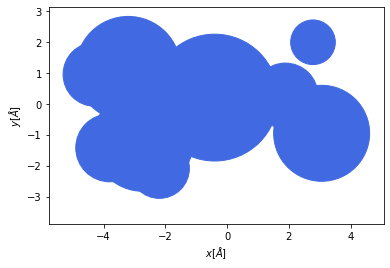
\includegraphics[width=0.5\textwidth]{figures/fourier/slice-iso.png} % for .pdf files etc use \includegraphics{test.pdf}
  \caption[Visualization of a slice with isolates]{A slice with isolates.}
  \label{fig:slice}
\end{figure}

%TODO: Not perfect, but good enough?
\paragraph{Finding the contour}

From the set of intersecting circles, the contour needs to be extracted. 
Since the contour points are computed just from radius and position information, and not rendered onto a 2D pixel grid, standard contour finding algorithms cannot be used.
Instead, knowledge about the general shape is used to compute the contour. 

The contour is computed using \autoref{alg:CircleSetContour}.

First, the point "furthest to the right", so with the largest $x$-Value is found. 
Since the point with the highest $x$-Value in any circle is always at angle 0, we set the initial angle $\alpha$ and rotation vector $\vec{p}$ accordingly.
From the circle containing that point, the contour is followed from that point counter-clockwise until the first intersection with another circle is found.
To the list of contour sections, the current contour section from angle $0$ to the angle of intersection is added.

Now, the contour of this circle is followed again until it intersects another.
This is repeated until the starting circle is reached again.

Once the starting circle is reached, the last remaining contour part of the starting circle needs to be added to the list of contour sections Figure~\ref{fig:circlesetcontour}.

From the ordered list of contour sections, the contour points can easily be computed.
Since each contour section consist of a radius $r$, location $(x,y)$, and start- and end angle $\alpha_{start}, \alpha_{end}$, the coordinates of the contour points can simply be computed using $x_c = \cos(\alpha_c) \cdot r + x$ and  $y_c = \sin(\alpha_c) \cdot r + y$ 
for $\alpha_c = \alpha_{start} + i \cdot \Delta, \alpha_c \leq \alpha_{end}, i \in \mathbb{N}_0$.

$\Delta$ is a tuning parameter that specifies the resolution of the contour.

This process is going along the outside ignores all "holes" in the shape, so only the outermost contour will be part of the final result. 
This is beneficial since EFDs only allow for the encoding of a single closed contour.

\begin{figure}[H]
  \minipage{0.32\textwidth}
    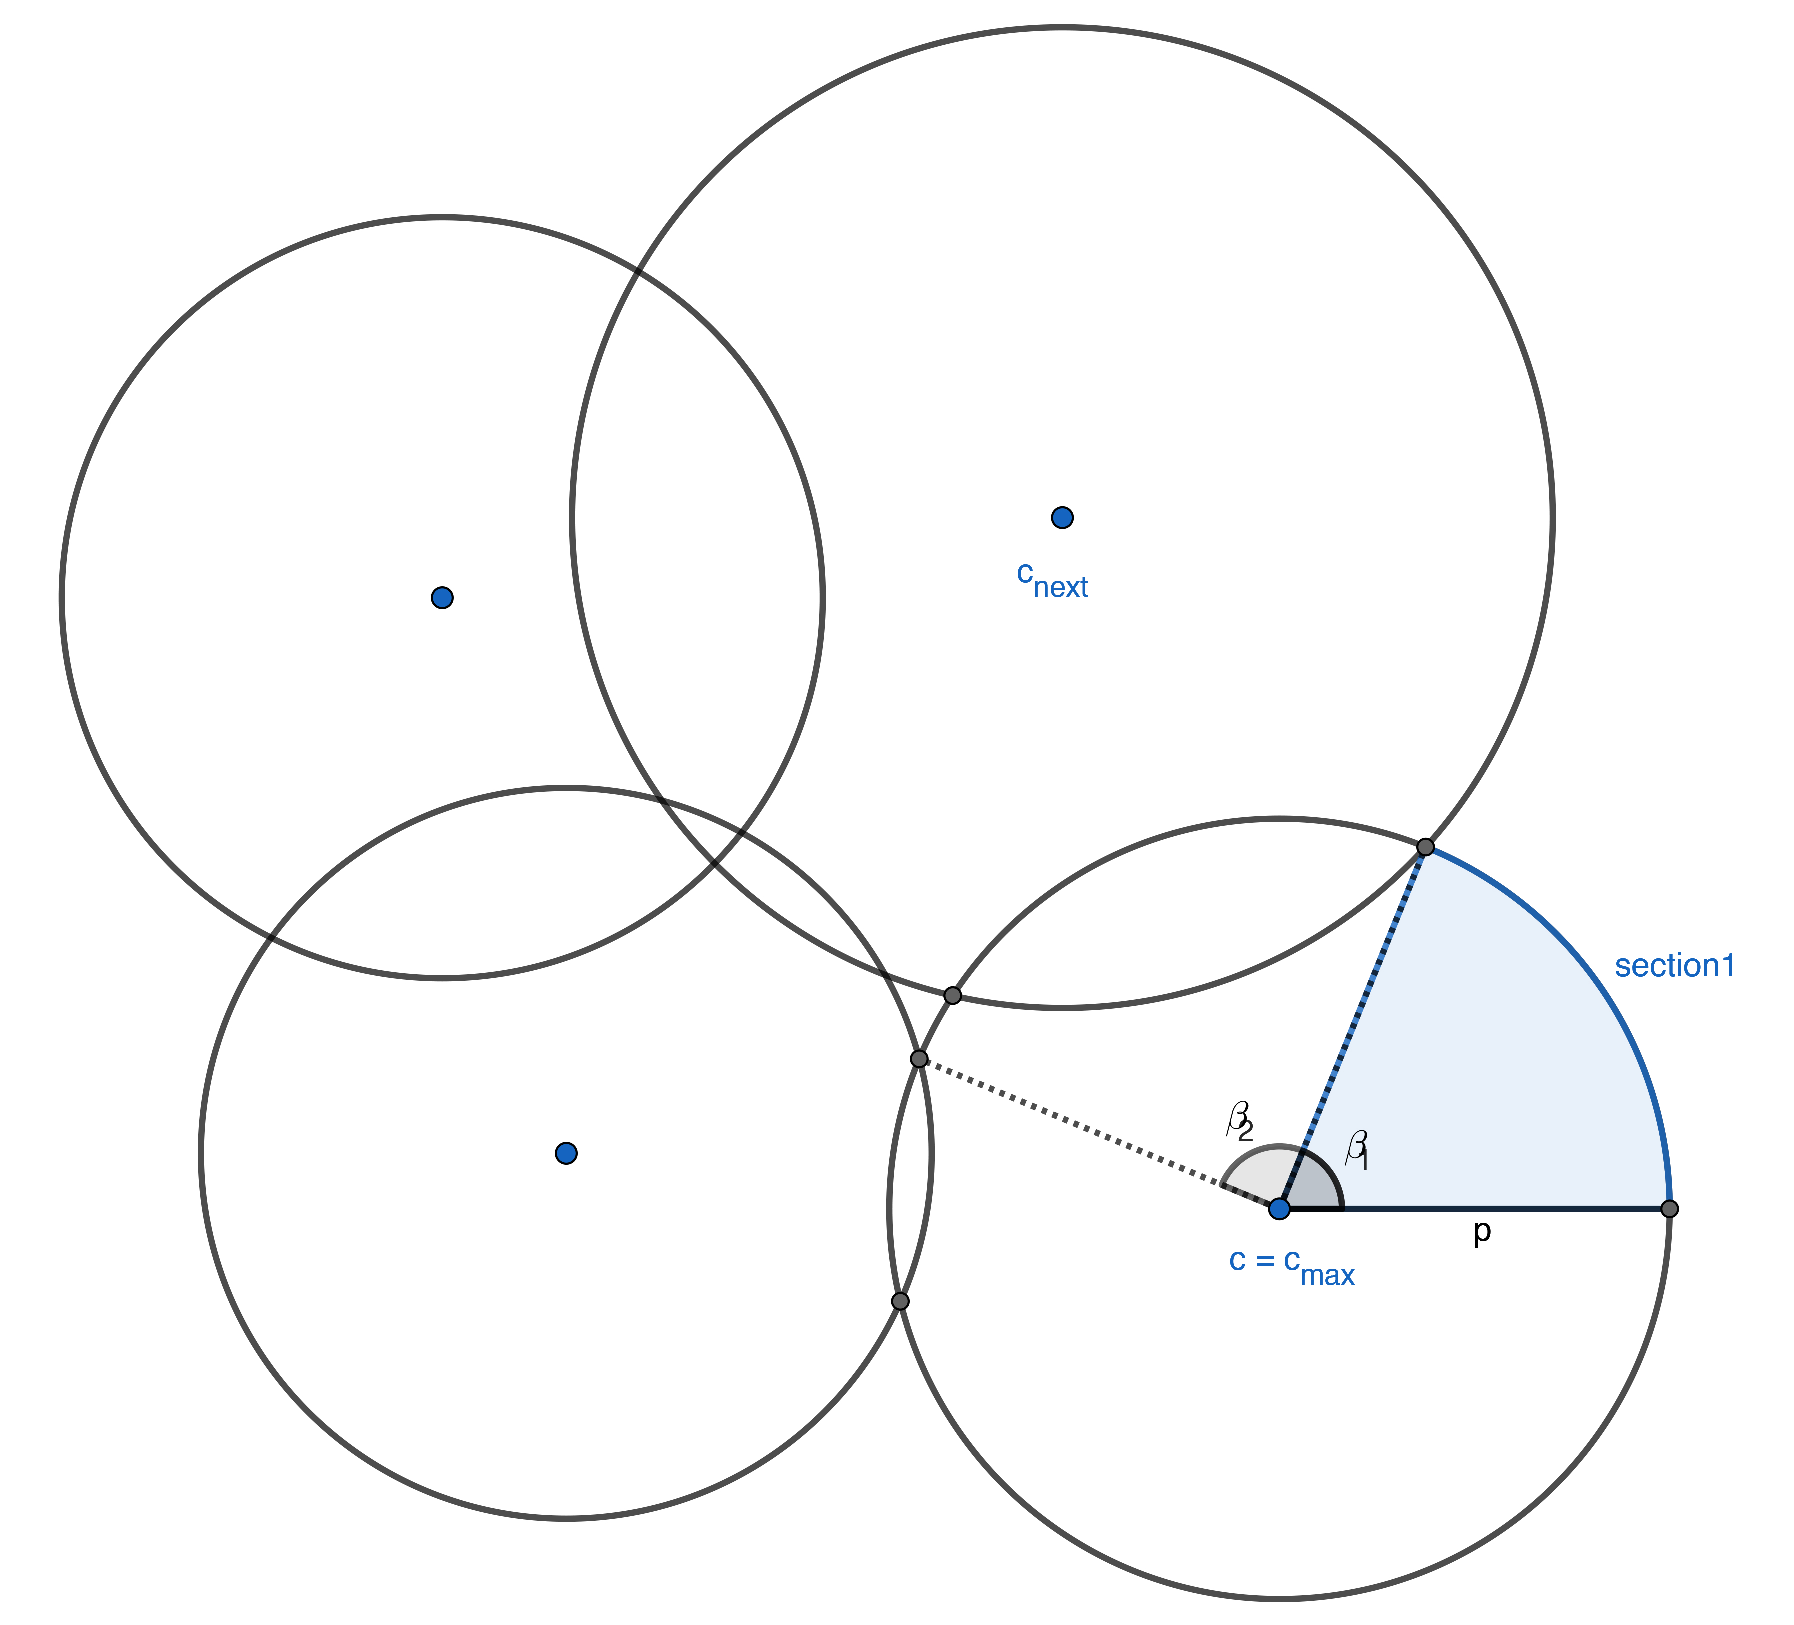
\includegraphics[width=1.0\textwidth]{figures/contour/c1copy.pdf}
    \caption{Finding first contour section}
  \endminipage\hfill
  \minipage{0.32\textwidth}
    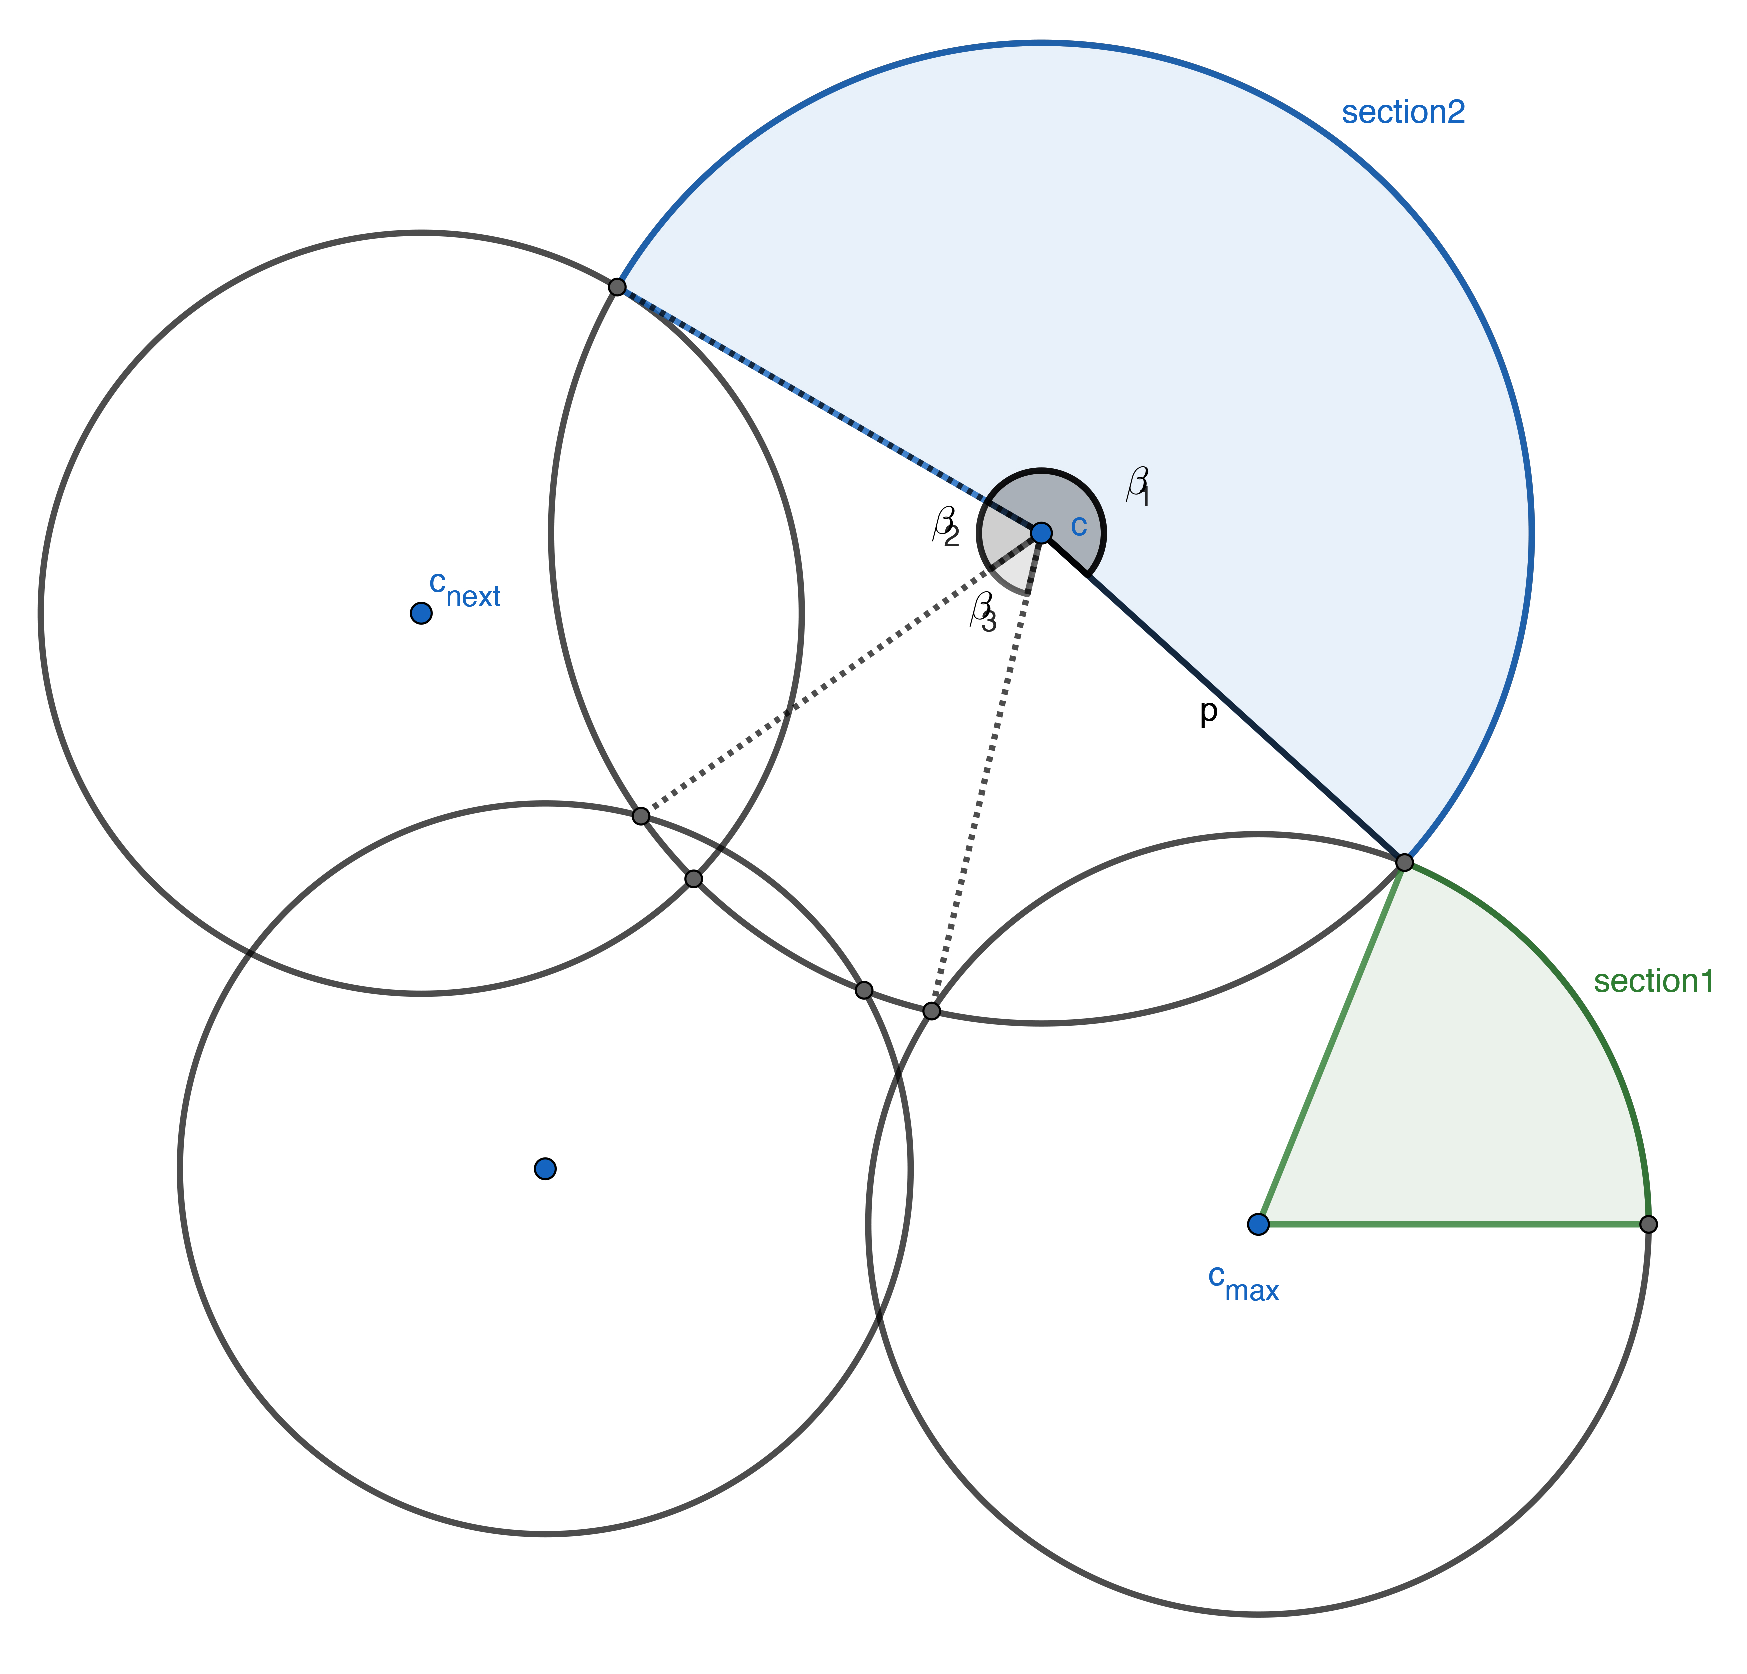
\includegraphics[width=1.0\textwidth]{figures/contour/c2copy.pdf}
    \caption{Finding middle contour section}
  \endminipage\hfill
  \minipage{0.32\textwidth}%
    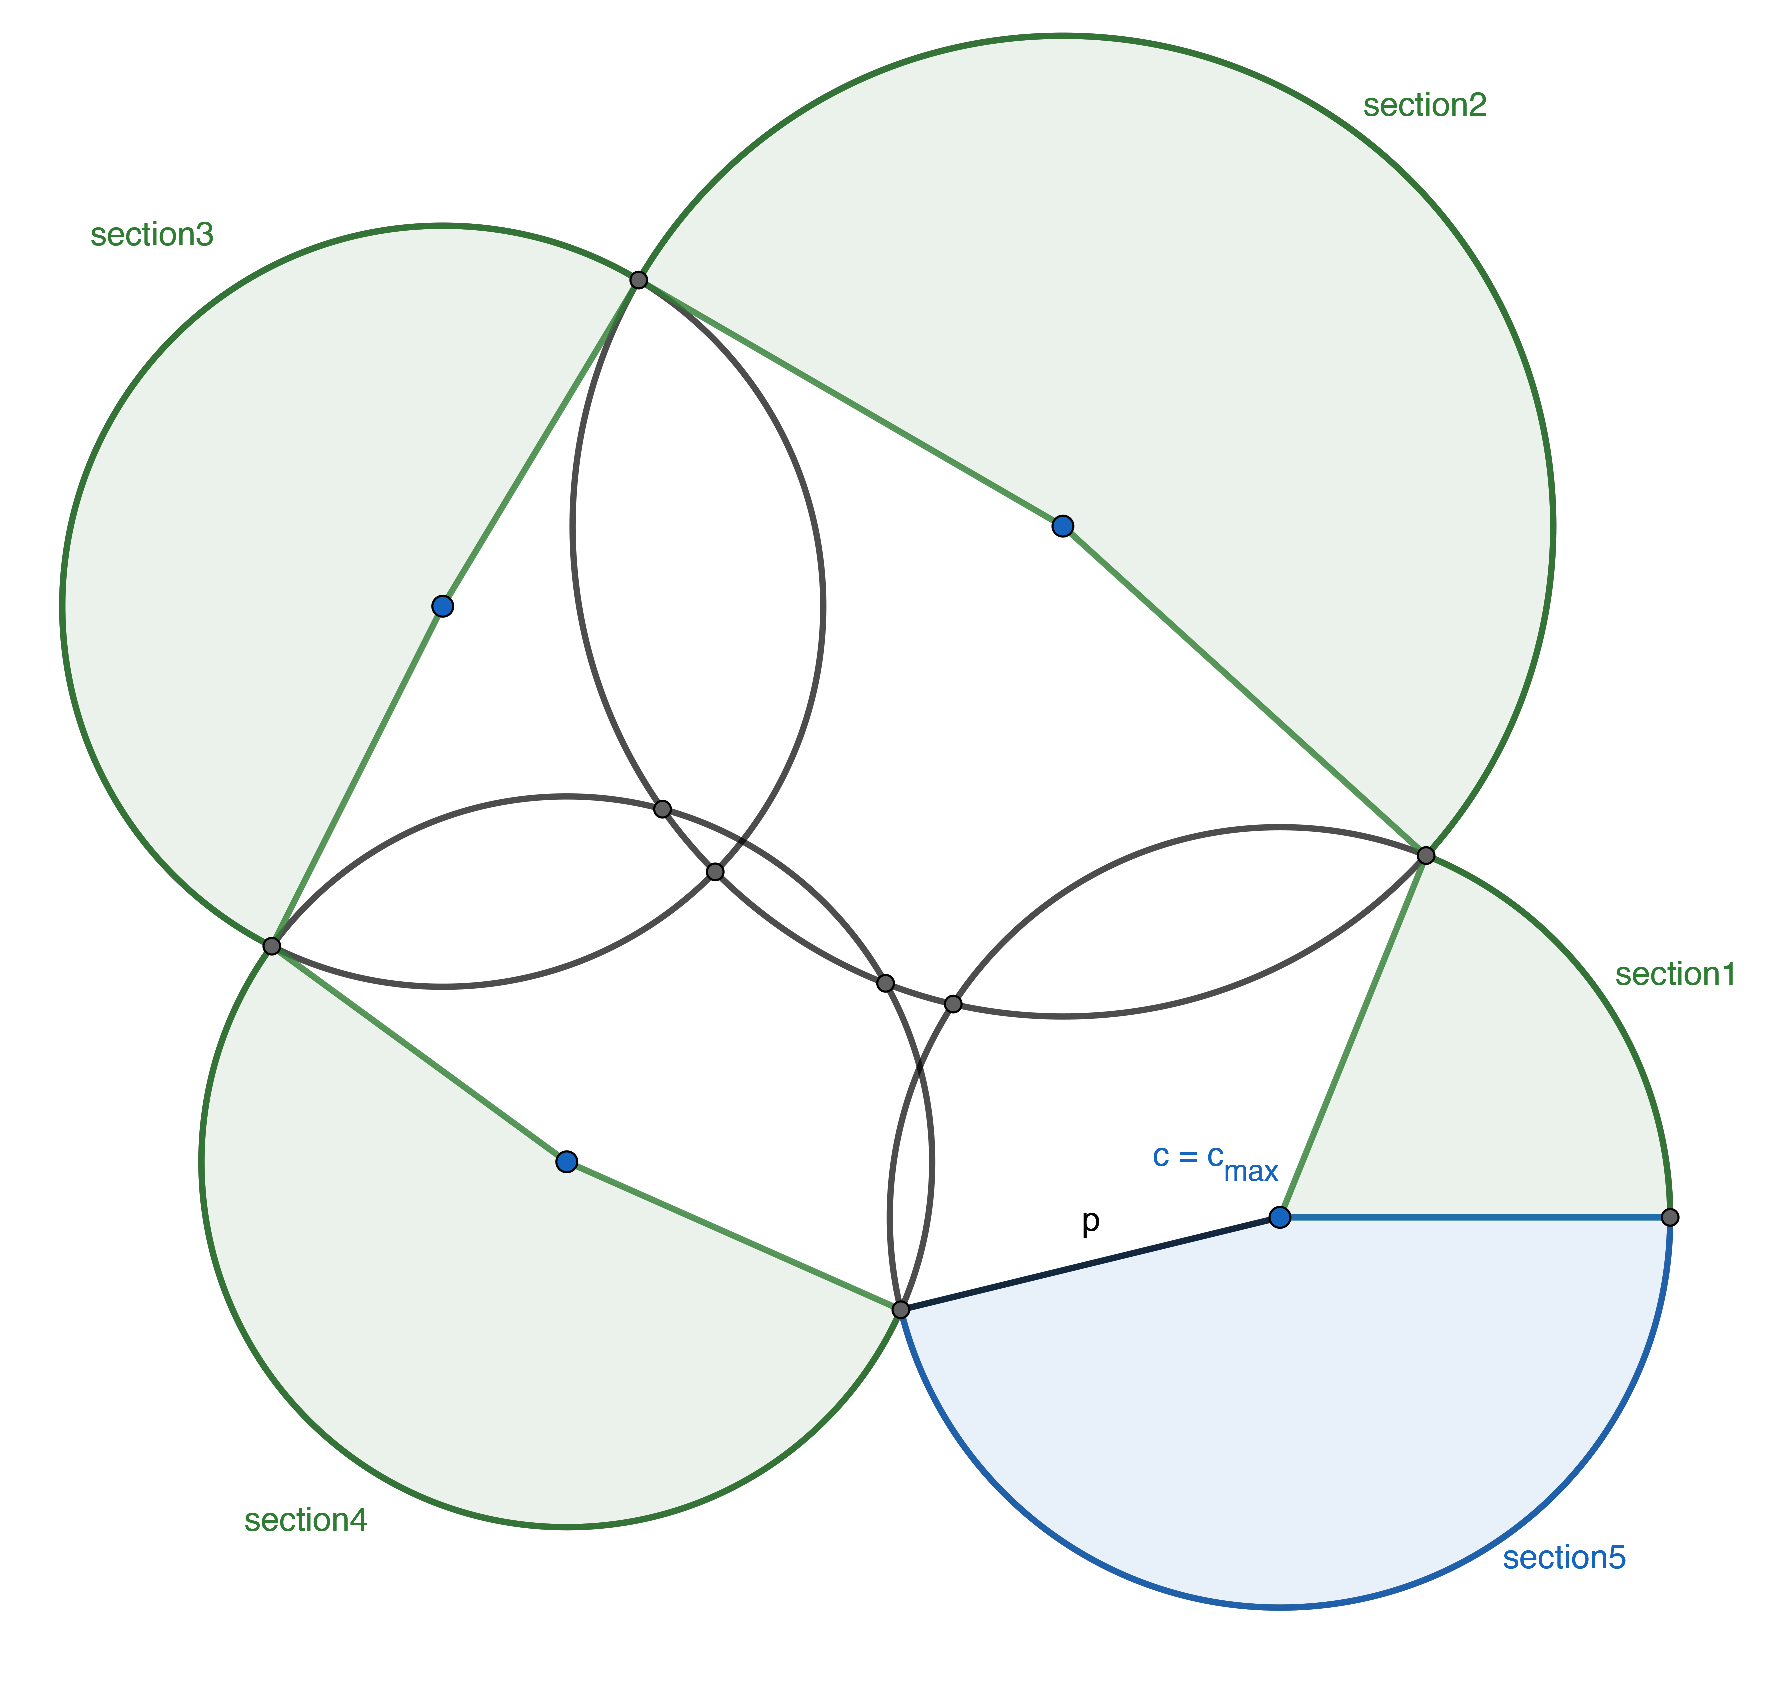
\includegraphics[width=1.0\textwidth]{figures/contour/c3copy.pdf}
    \caption{Finding the last contour section}
  \endminipage
  \caption[Visualization of CircleSetContour algorithm]{Visualization of \autoref{alg:CircleSetContour}}
  \label{fig:circlesetcontour}
\end{figure}


\subsection{Elliptic fourier descriptor}

Now that a contour for each slice is found, an elliptic fourier descriptor (EFD) will be used to describe that contour.
EFDs allow for a high resolution encoding of a contour in a fixed amount of coefficients.
Additionally, EFD coefficients can easily be made rotationally invariant.

EFDs, as described in \cite{LIN1987535} work by selecting a random starting point $s$ on the contour.
Starting from $s$, the contour will be followed. 
The $x$ and $y$ coordinates will be denoted as functions $x(l)$, $y(l)$ of the distance $l$ from the starting point.
Distance refers to the length it takes to get from $s$ to the point following the contour.

Since the starting and end point of $x(l), y(l)$ will be equal, making them periodic, a parameter $t=\frac{2\pi l}{n}$ can be defined. %TODO: Erklären!!!!
The functions can then be described by Fourier expansions as

%TODO: Replace t and put it in directly?
$$
\begin{pmatrix}
  x(l) \\
  y(l) \\
\end{pmatrix}
=
\begin{pmatrix}
  a_0 \\
  d_0 \\
\end{pmatrix}
+
\sum_{k=1}^\infty 
\begin{pmatrix}
  a_k & b_k\\
  c_k & d_k\\
\end{pmatrix}
\cdot
\begin{pmatrix}
  \cos(kt)\\
  \sin(kt)\\
\end{pmatrix}
$$

with

$$
a_0 = \frac{1}{2\pi} \int_{0}^{2 \pi}  x(t) \,dt 
$$
$$
d_0 = \frac{1}{2\pi} \int_{0}^{2 \pi}  y(t) \,dt 
$$

$$
a_k = \frac{1}{\pi} \int_{0}^{2 \pi}  x(t) \cos(kt) \,dt 
$$
$$
b_k = \frac{1}{\pi} \int_{0}^{2 \pi}  x(t) \sin(kt) \,dt 
$$
$$
c_k = \frac{1}{\pi} \int_{0}^{2 \pi}  y(t) \cos(kt) \,dt 
$$
$$
d_k = \frac{1}{\pi} \int_{0}^{2 \pi}  y(t) \sin(kt )\,dt 
$$

The $a_k, b_k, c_k, d_k$ form a basis for the functions $x(l), y(l)$.
By addition of the vector $ \begin{pmatrix} a_0 & b_0 \end{pmatrix}^T $ a center offset can be defined.
Since the contours encoded here should stay rotationally invariant, a two dimensional offset is not feasible.
Instead the offset length $\|  \begin{pmatrix} a_0 & b_0 \end{pmatrix}^T \| $ is added to the feature vector.

So far, the features $a_k, b_k, c_k, d_k$ are depended on the rotation of the contour.
The next step will be to make the features invariant under rotations.
%%%The starting point $s$ does not affect the coefficients as shown by \citeauthor{KUHL1982236}.

The contour can be viewed as a summation of ellipses of different size.
By aligning the first ellipse and rotating all other ellipses accordingly, the final output can be made invariant
of rotation \cite{MEBA}.

$$
\theta = \frac{1}{2}\arctan \left( \frac{2(a_1b_1 + c_1d_1)}{a_1^2 + c_1^2 - b_1^2 - d_1^2} \right)
$$
$$
\psi = \arctan \left( \frac{\cos(\theta) a_1 + \sin(\theta) b_1 }{\cos(\theta) c_1 + \sin(\theta) d_1} \right)
$$

The aligned coefficients $a_k^R, b_k^R, c_k^R, d_k^R$ can then be obtained using

$$
\begin{pmatrix}
  a_k^* & b_k^* \\
  c_k^* & d_k^* \\
\end{pmatrix}
=
\begin{pmatrix}
  \cos(\psi) & -\sin(\psi) \\
  \sin(\psi) & \cos(\psi) \\
\end{pmatrix}
\begin{pmatrix}
  a_k & b_k \\
  c_k & d_k \\
\end{pmatrix}
\begin{pmatrix}
  \cos(k\theta ) & -\sin(k\theta) \\
  \sin(k\theta) & \cos(k\theta) \\
\end{pmatrix}
$$.

The rotation around $\theta $ can be interpreted as normalizing the starting point $v$, 
the rotation around $\psi$ as normalizing the rotation of the contour itself \cite{KUHL1982236}.

The last step is to choose an order up to which the contour is approximated.
At the moment the infinite sum ensures a perfect approximation of the original contour. 
By limiting the coefficients to an order $k_{max}$ the number of coefficients describing our contour can be limited.
Generally, the higher the order, the better small changes in the contour can be approximated [Figure~\ref{fig:slice-layered}].


After normalizing, the values $b_1^* = c_1^* = 1$ will always be equal to 0, since the first ellipse as rotated to be aligned.
Therefore $b_1^*, c_1^*$ can be removed from the feature vector.

After calculating the coefficients for every slice, the different slices will be concatenated into a 2D array.
One dimension of the array will correspond to the spacial $z$ direction, so it will be equivalent to the number of layers chosen.
The other dimension will hold the fourier coefficients for each layer.
\begin{figure}[H]
  \minipage{0.4\textwidth}
    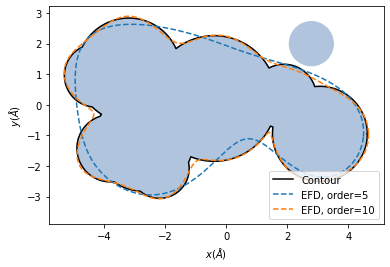
\includegraphics[width=1.0\textwidth]{figures/fourier/contour.png}
  \endminipage\hfill
  \minipage{0.6\textwidth}
    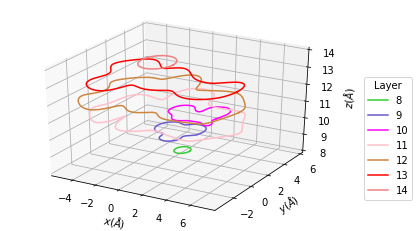
\includegraphics[width=1.0\textwidth]{figures/fourier/fourier-slices.png}
  \endminipage
  \caption[Slices produced by LEFD encoder]{
  On the left a slice is described by fourier descriptors. Higher order descriptors are able to approximate the contour better than lower order descriptors. 
  The isolate is ignored by the contour descriptor. The rotation is kept as part of the fourier description for illustration purposes.
  On the right the different slices making up on element are placed on top of each other. Slices without any volume are not rendered. 
  While the rotation is removed to keep it rotationally invariant, the offset from the center is encoded.
  }
  \label{fig:slice-layered}
\end{figure}

To keep information about the offset from the center, the length $l = \| \begin{pmatrix} a_0 & b_0 \end{pmatrix} \| $ will be added for each slice.
Since each fourier coefficient consists of 4 values and $b_1^*, c_1^*$ are removed while the center offset $l$ is added, the size of this dimension will be $k_{max} * 4 - 1$.

These features will be used for prediction of a molecules activation barrier in the next step.


\newpage
\section{Feature generation using smooth normalized atomic positions}
\label{ch:SNAP}
In a second approach, the molecule was encoded by smoothing the atomic positions, 
and then combining a set of functions describing the 3D space around the metal center.

This method is similar to the Smooth Overlap of Atomic Positions (SOAP) descriptor, that produces a 
fully rotational invariant description for the space surrounding one or more atomic centers \cite{Bart_k_2013}.
Specifically the gaussian smoothing of atomic positions and combination of radial basis functions with
spherical harmonics to describe a 3D space is taken from SOAP.
While SOAP describes the overlap of densities for different species, the goal here is to describe the density space directly.
The disadvantage of SOAP is that due to the rotational invariance, the 3D environment cannot be reconstructed from the generated features.
Due to the similarities between SOAP and SNAP, parts of the implementation and the following description of SNAP are based 
on the open-source library Dscribe that provides an implementation of SOAP \cite{dscribe}.

The Smooth Normalized Atomic Positions (SNAP) descriptor proposed here allows for a reconstruction of the 3D space from the coefficients, 
while partly keeping the rotational invariance.
Rotational invariance however is not given by the feature generation itself, but rather by using the catalysts special struture.
The SNAP descriptor therefore is less universal than SOAP. 
In applications were no translation back to 3D space is required,
in most instances SOAP should be chosen over SNAP for its fully rotationally invariant output.

\subsection{SNAP requirements}

The general idea of SNAP is to describe the atoms surrounding a cental atom using a fixed set of coefficients.
Rotational invariance therefore cannot be guaranteed, unless the encoded molecule itself can be rotated in a way to explicitly set it's rotation.

For catalyst molecules, this natural axis can be defined by setting the reaction pocket to the top, and the central iridium atom as a center.

For other molecule classes, defining a natural axis might not be as trivial.

When no clear axis of alignment can be found, the SNAP output may be augmented by rotating the input along all axis of freedom.
If there are multiple axis of freedom SOAP may be preferable since it naturally offers a fully rotationally invariant description.

Additionally, SNAP only encodes a local region within $r_{cut}$.
Density outside this cutoff radius is not considered.

If a global description of the entire element is needed, SNAP might not be the best option, especially when 
the size of the elements in the dataset varies a lot.

\subsection{SNAP}

Using the centered and aligned molecules, a density space surrounding the central iridium atom is defined.

By generating 3D gaussian distributions for every atom in the element, a density at any point within $r_{cut}$ can be calculated.
For each species $Z$ in the dataset, the density at any point $p = (x,y,z)$ is described as

$$\rho^Z(p) = \sum_i^{|Z|} w_{Z_i} e^{- \frac{1}{2\sigma^2} \vert p - R_i \vert^2 }$$  %TODO WAS IST SIGMA?

The summation $i$ runs over all the atoms of that species.
$R_i$ is the center of that atom.
$w_{Z_i}$ is a weight factor for each species. 
Since all species will be described independently of each other, for now all $w_{Z_i}=1$.
In further enhancements of the SNAP encoder, describing other molecular properties by adapting $w_{i}$ or the decay parameter $\sigma$ is possible.
Even describing 3D features not associated with a single species but rather describing the interaction or overlap of species 
or molecules are thinkable.

\begin{figure} [H]
  \centering
  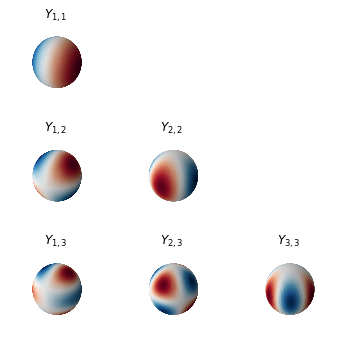
\includegraphics[width=0.5\textwidth]{figures/snap/sph-harm.png} % for .pdf files etc use \includegraphics{test.pdf}
  \caption[Spherical harmonics]{A selection of low order spherical harmonics plotted on a sphere. } %TODO: Add scale!!!
  \label{fig:sphharm}
\end{figure}

Since the basis set used to describe the space is using spherical coordinates, from now on
cartesian coordinates will be replaced by spherical coordinates.

$$
r = \sqrt{x^2 + y^2 + z^2}
,
\theta = \arccos(\frac{z}{r})
,
\varphi = \arctan(y / x)
$$ %TODO: Überprüfen

The density space can then be expanded using a combination of basis functions.
To expand the radial degrees of freedom, spherical harmonics are used.
Spherical harmonics are a complete set of orthonormal basis functions on spherical coordinates.
The spherical harmonics used here are the Laplacian Spherical Harmonics.
$$
Y_{lm}(\theta, \varphi) = (-1)^m \sqrt{\frac{2l + 1}{4 \pi} \frac{(l - m)!}{(l + m)!}} P_{lm}\left(\cos(\theta) \right) e^{im\theta}
$$

Here, $P_{lm}$ are the associated Legendre polynomials:

$$
P_{lm}(x) = (-1)^m (1-x^2)^{m/2} \frac{\partial^{l+m}}{\partial x^{l+m}}(x^2 - 1)^l
$$ %TODO: Looks at derivative



Using the spherical harmonics, a sphere surrounding the central atom can be encoded.
To encode density information along the radial direction, spherical harmonics are combined with radial basis functions.
A variety of radial functions can be used for this application.
In \cite{KUHL1982236} the use of a polynomial radial basis is suggested.
However here a set of primitive gaussian type orbitals are used.
This set allows for analytical integration which allows for a significant speedup over numerical integration since it can be precomputed \cite{dscribe}.
These gaussian type orbitals are defined as

$$g_{nl}(r) = \sum_{n'}{n_{max}} \beta_{nn'l} \phi_{n'lr}(r) $$

with 

$$\phi_{nl}(r) = r^l e^{-\alpha_{nl}r^2} $$ %TODO: phi of n oder phi of nl?? / alpha_n oder alpha_nl



$\alpha$ and $\beta$ are constants that only need to be computed once for every pair of $l,m, r_{cut}$.
The $\alpha$ parameters control the decay of the radial basis functions at $r_{cut}$.

\begin{figure} [hb!]
  \centering
  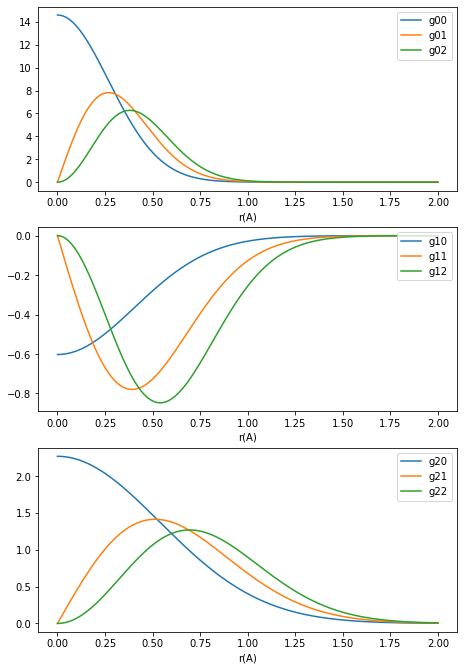
\includegraphics[width=0.5\textwidth]{figures/snap/gaus_orb.png} % for .pdf files etc use \includegraphics{test.pdf}
  \caption[Radial basis functions]{Spherical gaussian orbital functions for a cutoff radius $r_{cut}=2$, $2$, $n_{max}=2$ and $l_{max}=2$. }
  \label{fig:gaussians}
\end{figure}

$\beta_{nn'l}$ parameters orthogonalize the radial basis functions.
For each $l$ the weights $\beta_{nn'l}$ can be computed using the Löwdin orthogonalization:

$$\beta = S(l)^{-1/2} $$

with the entries of the matrix $S$ being defined as

$$S(l)_{nn'} = \langle \phi_{nl} | \phi_{n'l} \rangle  $$

The implementation of $\alpha$ and $\beta$ prefactors is taken from \cite{dscribe} where they are precomputed up to $l \leq 9$.
Higher order factors could be added if needed.


Combining spherical harmonics with radial basis functions the density space surrounding the central atom can be described.
In theory, choosing infinitely high $n, l$ could approximate the space with infinitely high precision.
To get a fixed amount of coefficients, $n_{max}$ and $l_{max}$ need to be chosen that determine the
accuracy of the encoding.
Generally, the higher $n_{max}, l_{max}$ the more accurate the space can be approximated.
%TODO Add figure of the space being described with different n, l , cutoff

For radial basis functions a cutoff radius $r_{cut}$ needs to be defined.
Densities outside this cutoff radius will not be encoded in the features of the space.

The density for every species $Z$ in within the cutoff sphere can be expanded as:

$$ \rho^Z(r) = \sum_{nlm} c^Z_{nlm} g_{nl}(r) Y_{lm}(\theta, \varphi) $$

The coefficients $c_{nlm}^Z$ are features generated by the SNAP descriptor.

$$ c_{nlm}^Z = \iiint_{R^3} g_{nl}(r) Y_{lm}(\theta, \varphi) \rho^Z(r, \theta, \phi)  \,dr\theta\phi   $$
% TODO: Integrate to infinity or r_cut?

The 3 dimensional integral goes over all spherical coordinates within the cutoff sphere.
The coefficients $c^Z_{nlm}$ now describe the 3D space within a fixed size sphere.
\\
The key difference between SNAP and other chemical descriptors is the bi-directional mapping between feature space and 
density space.
From the coefficients, the density space can be easily reconstructed.
This allows for a partial reconstruction of the molecule from the features encoded by SNAP.

However, due to the low number of radial basis functions and spherical harmonics usually used to describe an element, 
the encoding of the density is far from perfect.
With an infinite amount of coefficients a perfect description of the space is thinkable,
in reality computational limits only allow for a rather low resolution of the density space [Figure~\ref{fig:snap-density}]. 
\begin{figure} [h]
  \centering
  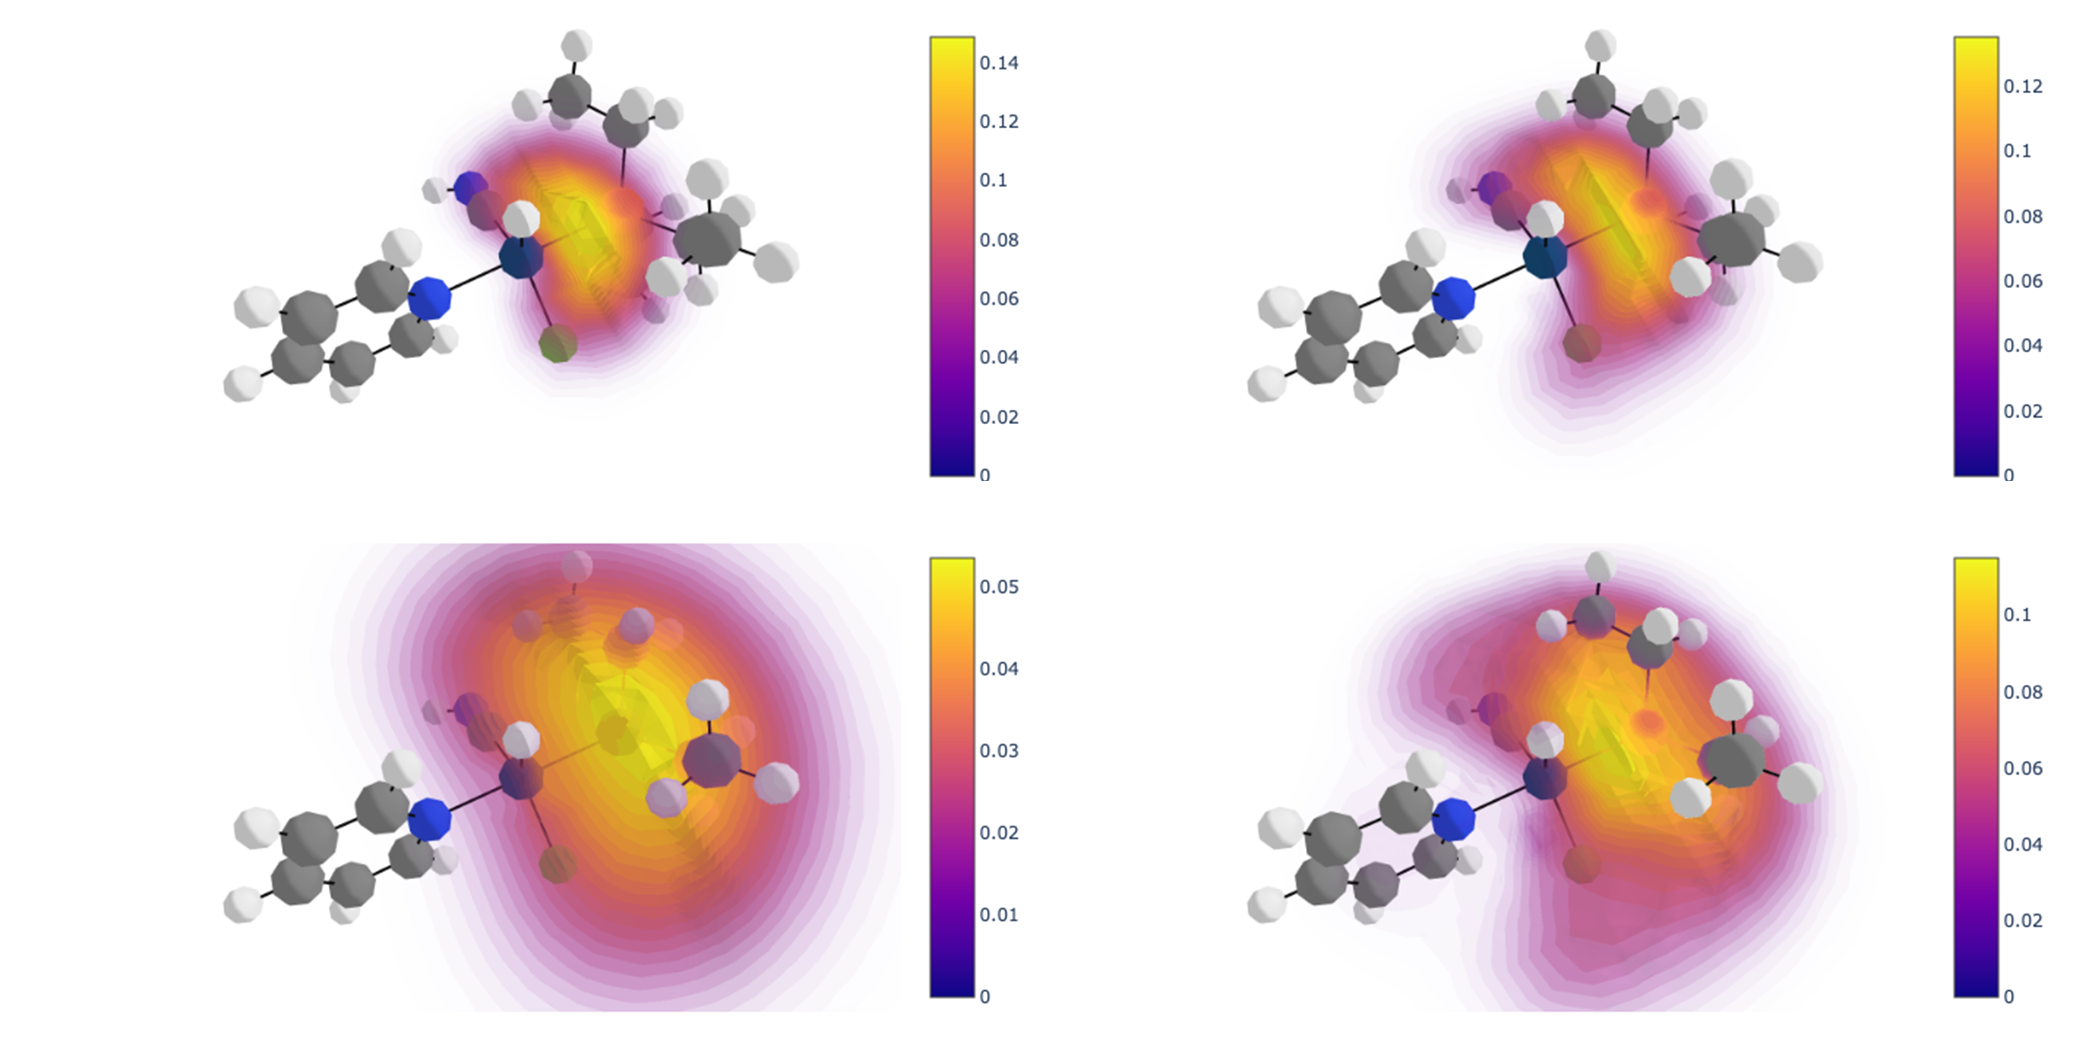
\includegraphics[width=1\textwidth]{figures/snap/density/dense.png} % for .pdf files etc use \includegraphics{test.pdf}
  \caption[SNAP density visualization]{Visualization of the density reconstructed from $c_{nlm}^Z$ coefficients for different resolutions.
  Top: $r_{cut} = 10$, bottom: $r_{cut} = 25$, left: $n_{max} = l_{max} = 2$, right: $n_{max} = l_{max} = 8$.
  The density shown is visualizing the density for phosphorus only.
  The phosphorus atom is the orange atom surrounded by the density cloud.
  }
  \label{fig:snap-density}
\end{figure}

This means that in many cases, the center of the encoded density and the center of the atom do not match.
Especially when the element contains many atoms of one species, the descriptor struggles to fully encode the space.

Despite these issues, predicting the activation barrier from SNAP features is still possible with high accuracy.
The interpretability of these results however is limited to a low resolution.
When using network explainers in combination with SNAP coefficients, this limited accuracy needs to be kept in mind.
